\subsection{Design}

Klient og server kommunikerer med hinanden vha. en række besked objekter. Strukturen af disse er udarbejdet efter følgende diagrammer.

Nedarving fra message klassen er vist på figur~\ref{fig:MessageUML}
\begin{figure}
	\centering
	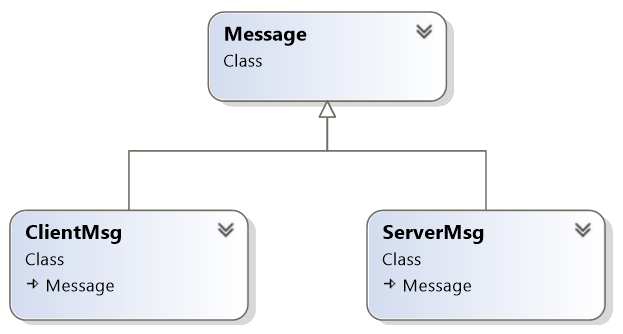
\includegraphics[width=0.6\linewidth]{figs/connection/MessageUML.png}
	\caption{Message nedarving}
	\label{fig:MessageUML}
\end{figure}

Nedarving fra ClientMsg klassen er vist på figur~\ref{fig:ClientMsgUML}
\begin{figure}
	\centering
	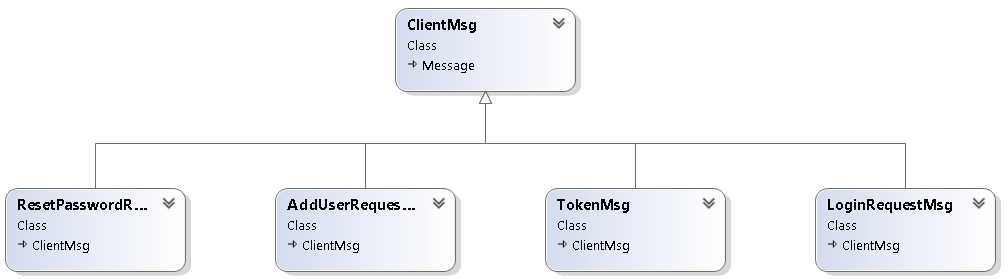
\includegraphics[width=0.9\linewidth]{figs/connection/ClientMsgUML.png}
	\caption{ClientMsg nedarving}
	\label{fig:ClientMsgUML}
\end{figure}

Nedarving fra TokenMsg er vist på figur~\ref{fig:TokenMsgUML}. AddPoolPictureRequestMsg er ikke blevet implementeret, men var en del af de user stories som blev udvalgt i starten af projektet, og er derfor taget med på figuren.
\begin{figure}
	\centering
	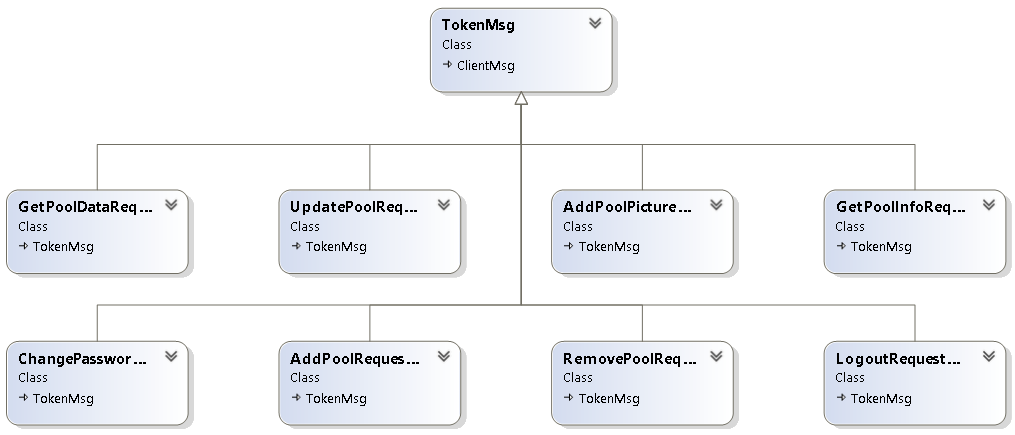
\includegraphics[width=0.9\linewidth]{figs/connection/TokenMsgUML.png}
	\caption{TokenMsg nedarving}
	\label{fig:TokenMsgUML}
\end{figure}

Nedarving fra ServerMsg er vist på figur~\ref{fig:ServerMsgUML}
\begin{figure}
	\centering
	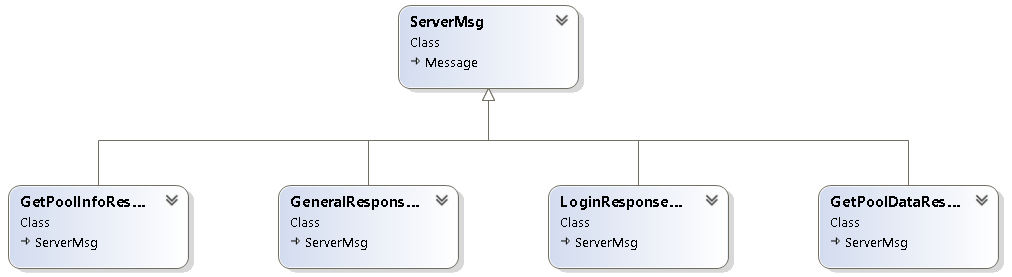
\includegraphics[width=0.9\linewidth]{figs/connection/ServerMsgUML.png}
	\caption{ServerMsg nedarving}
	\label{fig:ServerMsgUML}
\end{figure}

\subsection{Implementering}
Beskeder i systemet foregår via en række objekter, der alle nedarver fra en basis klasse ved navn Message. Disse er beskrevet nærmere i følgende afsnit

\subsubsection{Message}
Indeholder en enum af typen MessageTypes, hvori alle typer beskeder fremgår. Desuden indeholder den en string med MessageInfo, som primært anvendes i tilfælde af fejl, hvor beskeden vises i systemets GUI som vist på figur~\ref{fig:loginError}

\begin{figure}
	\centering
	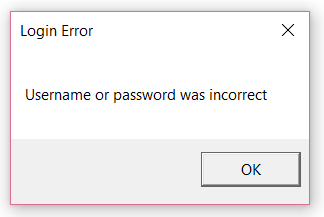
\includegraphics[width=0.3\linewidth]{figs/connection/loginError.png}
	\caption{Login error}
	\label{fig:loginError}
\end{figure}

\subsubsection{ClientMsg}
Indeholder ikke yderligere informationer, men definerer en adskillelse mellem server beskeder og klient beskeder. Desuden giver det mulighed for at alle klient beskeder i fremtiden kan indeholder informationer, som server beskeder ikke indeholder. 

\paragraph{ResetPasswordRequestMsg}
Denne beskedtype er ikke blevet færdigt implementeret. Beskeden var tiltænkt at skulle sende en mail til brugeren med et nyt password, men blev nedprioriteret pga. tidsmangel.
\begin{lstlisting}[caption=ResetPasswordRequestMsg, label=code:ResetPasswordRequestMsg]
public class ResetPasswordRequestMsg : ClientMsg
{
	public string Username { get; set; }
	
	public ResetPasswordRequestMsg(string username)
	{
		Username = username;
		MsgType = MessageTypes.ResetPasswordRequest;
	}
}
\end{lstlisting}

\paragraph{AddUserRequestMsg}
Indeholder de informationer der bliver gemt i databasen når en bruger bliver oprettet.
\begin{lstlisting}[caption=AddUserRequestMsg, label=code:AddUserRequestMsg]
public class AddUserRequestMsg : ClientMsg
{
	public string Fullname { get; set; }
	public string Username { get; set; }
	public string Password { get; set; }
	
	public AddUserRequestMsg(string fullname, string username, string password)
	{
		Fullname = fullname;
		Username = username;
		Password = password;
		MsgType = MessageTypes.AddUserRequest;
	}
}
\end{lstlisting}

\paragraph{LoginRequestMsg}
Indeholder informationer til at kontrollere om brugeren har indtastet det korrekte password
\begin{lstlisting}[caption=LoginRequestMsg, label=code:LoginRequestMsg]
public class LoginRequestMsg : ClientMsg
{
	public string Username { get; set; }
	public string Password { get; set; }
	
	public LoginRequestMsg(string username, string password)
	{
		Username = username;
		Password = password;
		MsgType = MessageTypes.LoginRequest;
	}
}
\end{lstlisting}

\subsubsection{TokenMsg}
Alle beskedtyper som kræver at brugeren er logget ind, nedarver fra denne besked. Beskeden indeholder udover en MsgType også en SubMsgType, til at definere hvilken nedarving af TokenMsg der er tale om. Dette er lavet så alle nedarvinger beholder typen TokenMsg som deres MsgType.
\begin{lstlisting}[caption=TokenMsg, label=code:TokenMsg]
public class TokenMsg : ClientMsg
{
	public string Username { get; set; }
	public string TokenString { get; set; }
	public TokenSubMessageTypes SubMsgType { get; set; }
	
	public TokenMsg(string username, string tokenString)
	{
		Username = username;
		TokenString = tokenString;
		MsgType = MessageTypes.TokenMsg;
	}
}
\end{lstlisting}

\paragraph{AddPoolRequest}
Indeholder informationer til at beskrive brugerens pool i systemet.
\begin{lstlisting}[caption=AddPoolRequest, label=code:AddPoolRequest]
public class AddPoolRequestMsg : TokenMsg
{
	public string PoolName { get; set; }
	public double Volume { get; set; }
	public string SerialNumber { get; set; }
	
	public AddPoolRequestMsg(string username, string tokenString, string poolName, double poolVolume, string serialNumber) : base(username, tokenString)
	{
		PoolName = poolName;
		Volume = poolVolume;
		SerialNumber = serialNumber;
		SubMsgType = TokenSubMessageTypes.AddPoolRequest;
	}
}
\end{lstlisting}

\paragraph{GetPoolDataRequest}
Indeholder informationer om hvilke data der ønskes modtaget i klienten. Beskeden kan oprettes med propperty GetAllNamesOnly sat til true, hvis klienten kun ønsker at modtage en liste med navne over alle pools brugeren har tilknyttet. Denne liste vil yderligere indeholde en bool for hver pool, som er true hvis en eller flere måleværdier er udenfor deres target værdi. En anden mulighed at angive et pool navn, hvilket resulterer i et svar med informationer om konkrete målinger, indenfor en tidsperiode der svarer til det angivne antal dage.
\begin{lstlisting}[caption=GetPoolDataRequest, label=code:GetPoolDataRequest]
public class GetPoolDataRequestMsg : TokenMsg
{
	public bool GetAllNamesOnly { get; set; }
	public string PoolName { get; set; }
	public int GetHistoryDays { get; set; }
	
	public GetPoolDataRequestMsg(string username, string tokenString, bool getAllNamesOnly = false, string poolName = "", int getHistoryDays = 0)
	: base(username, tokenString)
	{
		GetAllNamesOnly = getAllNamesOnly;
		PoolName = poolName;
		GetHistoryDays = getHistoryDays;
		SubMsgType = TokenSubMessageTypes.GetPoolDataRequest;
	}
}
\end{lstlisting}

\paragraph{GetPoolInfoRequest}
Indeholder navnet på den pool der ønskes information om, så som pool volume og serial number.
\begin{lstlisting}[caption=GetPoolInfoRequest, label=code:GetPoolInfoRequest]
public class GetPoolInfoRequestMsg : TokenMsg
{
	public string PoolName { get; set; }
	
	public GetPoolInfoRequestMsg(string username, string tokenString, string poolName) : base(username, tokenString)
	{
		PoolName = poolName;
		SubMsgType = TokenSubMessageTypes.GetPoolInfoRequest;
	}
}
\end{lstlisting}

\paragraph{RemovePoolRequest}
Indeholder navnet på den pool, brugeren ønsker at fjerne.
\begin{lstlisting}[caption=RemovePoolRequest, label=code:RemovePoolRequest]
public class RemovePoolRequestMsg : TokenMsg
{
	public string PoolName { get; set; }
	
	public RemovePoolRequestMsg(string username, string tokenString, string poolName) : base(username, tokenString)
	{
		PoolName = poolName;
		SubMsgType = TokenSubMessageTypes.RemovePoolRequest;
	}
}
\end{lstlisting}

\paragraph{UpdatePoolRequest}
Indeholder informationer som giver brugeren mulighed for at ændre en pools navn eller volume.
\begin{lstlisting}[caption=UpdatePoolRequest, label=code:UpdatePoolRequest]
public class UpdatePoolRequestMsg : TokenMsg
{
	public string OldPoolName { get; set; }
	public string NewPoolName { get; set; }
	public double NewPoolVolume { get; set; }
	
	public UpdatePoolRequestMsg(string username, string tokenString, string oldPoolName, string newPoolName = "", double newPoolVolume = 0) : base(username, tokenString)
	{
		OldPoolName = oldPoolName;
		NewPoolName = newPoolName;
		NewPoolVolume = newPoolVolume;
		SubMsgType = TokenSubMessageTypes.UpdatePoolRequest;
	}
}
\end{lstlisting}

\paragraph{ChangePasswordRequest}
Indholder informationer om brugerens gamle password, samt hvilket password brugeren fremover ønsker at benytte.
\begin{lstlisting}[caption=ChangePasswordRequest, label=code:ChangePasswordRequest]
public class ChangePasswordRequestMsg : TokenMsg
{
	public string OldPassword { get; set; }
	public string NewPassword { get; set; }
	
	public ChangePasswordRequestMsg(string username, string tokenString, string oldPassword, string newPassword) : base(username, tokenString)
	{
		OldPassword = oldPassword;
		NewPassword = newPassword;
		SubMsgType = TokenSubMessageTypes.ChangePasswordRequest;
	}
}
\end{lstlisting}

\paragraph{LogoutRequest}
Indeholder ikke yderligere informationer, da klassen allerede nedarver fra TokenMsg og dermed har username som en del af beskeden.
\begin{lstlisting}[caption=LogoutRequest, label=code:LogoutRequest]
public class LogoutRequestMsg : TokenMsg
{
	public LogoutRequestMsg(string username, string tokenString) : base(username, tokenString)
	{
		SubMsgType = TokenSubMessageTypes.LogoutRequest;
	}
}
\end{lstlisting}

\subsubsection{ServerMsg}
Denne klasse indeholder ikke yderligere informationer, men definerer en række beskeder som serveren kan svare med. Det er forsøgt at holde antallet af beskeder så lavt som muligt, ved f.eks. at lave en GeneralResponseMsg som anvendes på alle requests, hvor applikationen ikke modtager data, men blot ønsker at vide om den pågældende request blev udført. 

\paragraph{GeneralResponseMsg}
Indeholder informationer om hvor vidt en request blev udført. Der gives yderligere information om det skyldes at brugerens session ikke længere er aktiv, eller at det var selve requesten der fejlede.
\begin{lstlisting}[caption=GeneralResponseMsg, label=code:GeneralResponseMsg]
public class GeneralResponseMsg : ServerMsg
{
	public bool TokenStillActive { get; set; }
	public bool RequestExecutedSuccesfully { get; set; }
	public GeneralResponseMsg(bool tokenStillActive, bool requestExecutedSuccesfully)
	{
		TokenStillActive = tokenStillActive;
		RequestExecutedSuccesfully = requestExecutedSuccesfully;
		MsgType = MessageTypes.GeneralResponse;
	}
}
\end{lstlisting}

\paragraph{GetPoolDataResponse}
Indeholder enten informationer om alle poolnavne til en bruger, eller sensor målinger for en enkelt pool.
\begin{lstlisting}[caption=GetPoolDataResponse, label=code:GetPoolDataResponse]
public class GetPoolDataResponseMsg : ServerMsg
{
	public List<Tuple<SensorTypes, List<double>>> SensorList { get; set; }
	public List<Tuple<string, bool>> AllPoolNamesListTuple { get; set; }
	
	public GetPoolDataResponseMsg(List<Tuple<SensorTypes, List<double>>> sensorList = null, List<Tuple<string, bool>> allPoolNamesListTuple = null )
	{
		SensorList = sensorList;
		AllPoolNamesListTuple = allPoolNamesListTuple;
		MsgType = MessageTypes.GetPoolDataResponse;
	}
}
\end{lstlisting}

\paragraph{GetPoolInfoResponse}
Indeholder informationer om en brugers pool
\begin{lstlisting}[caption=GetPoolInfoResponse, label=code:GetPoolInfoResponse]
public class GetPoolInfoResponseMsg : ServerMsg
{
	public double Volume { get; set; }
	public string SerialNumber { get; set; }
	
	public GetPoolInfoResponseMsg(double volume, string serialNumber)
	{
		Volume = volume;
		SerialNumber = serialNumber;
		MsgType = MessageTypes.GetPoolInfoResponse;
	}
}
\end{lstlisting}

\paragraph{LoginResponse}
Indeholder informationer om hvor vidt det lykkedes at logge ind på systemet. Hvis login lykkedes, vil beskeden også indeholde en TokenString, som applikationen derefter sender med fremtidige requests.
\begin{lstlisting}[caption=LoginResponse, label=code:LoginResponse]
public class LoginResponseMsg : ServerMsg
{
	public string TokenString { get; set; }
	public bool LoginSuccessful { get; set; }
	
	public LoginResponseMsg(string tokenString, bool loginSuccessful)
	{
		TokenString = tokenString;
		LoginSuccessful = loginSuccessful;
		MsgType = MessageTypes.LoginResponse;
	}
}
\end{lstlisting}